\chapter{Исследовательская часть}

\section{Среда для тестирования}

Для тестирования разработанного алгоритма применялась облачная платформа Google Colab, не требующая установки ПО на локальный компьютер.

\section{Использование ReLu в качестве функции активации}

\begin{figure}
	\begin{center}
		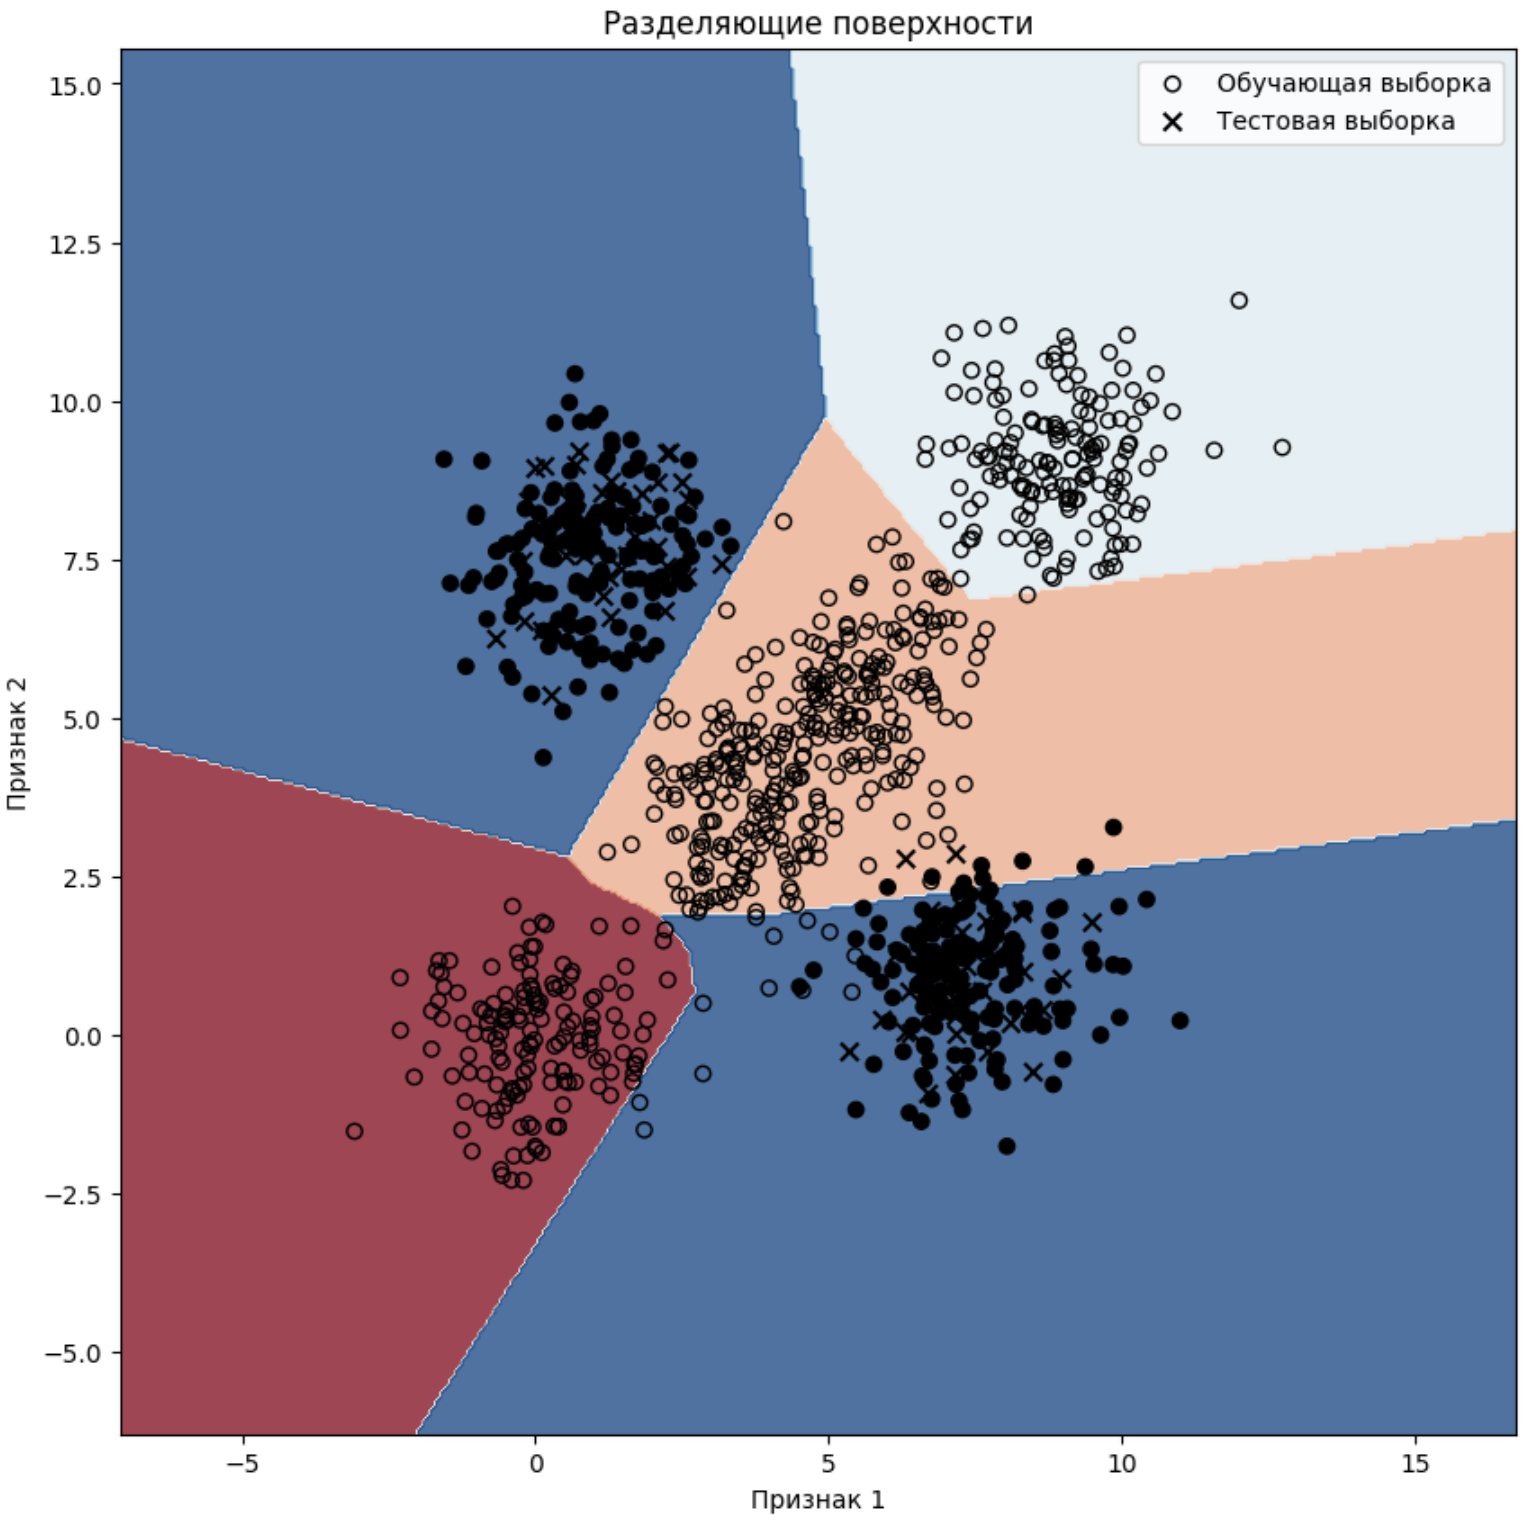
\includegraphics[width=\textwidth]{images/1.png}
	\end{center}
	\caption{Разделяющие поверхности}
	\label{img:1}
\end{figure}

\begin{figure}
	\begin{center}
		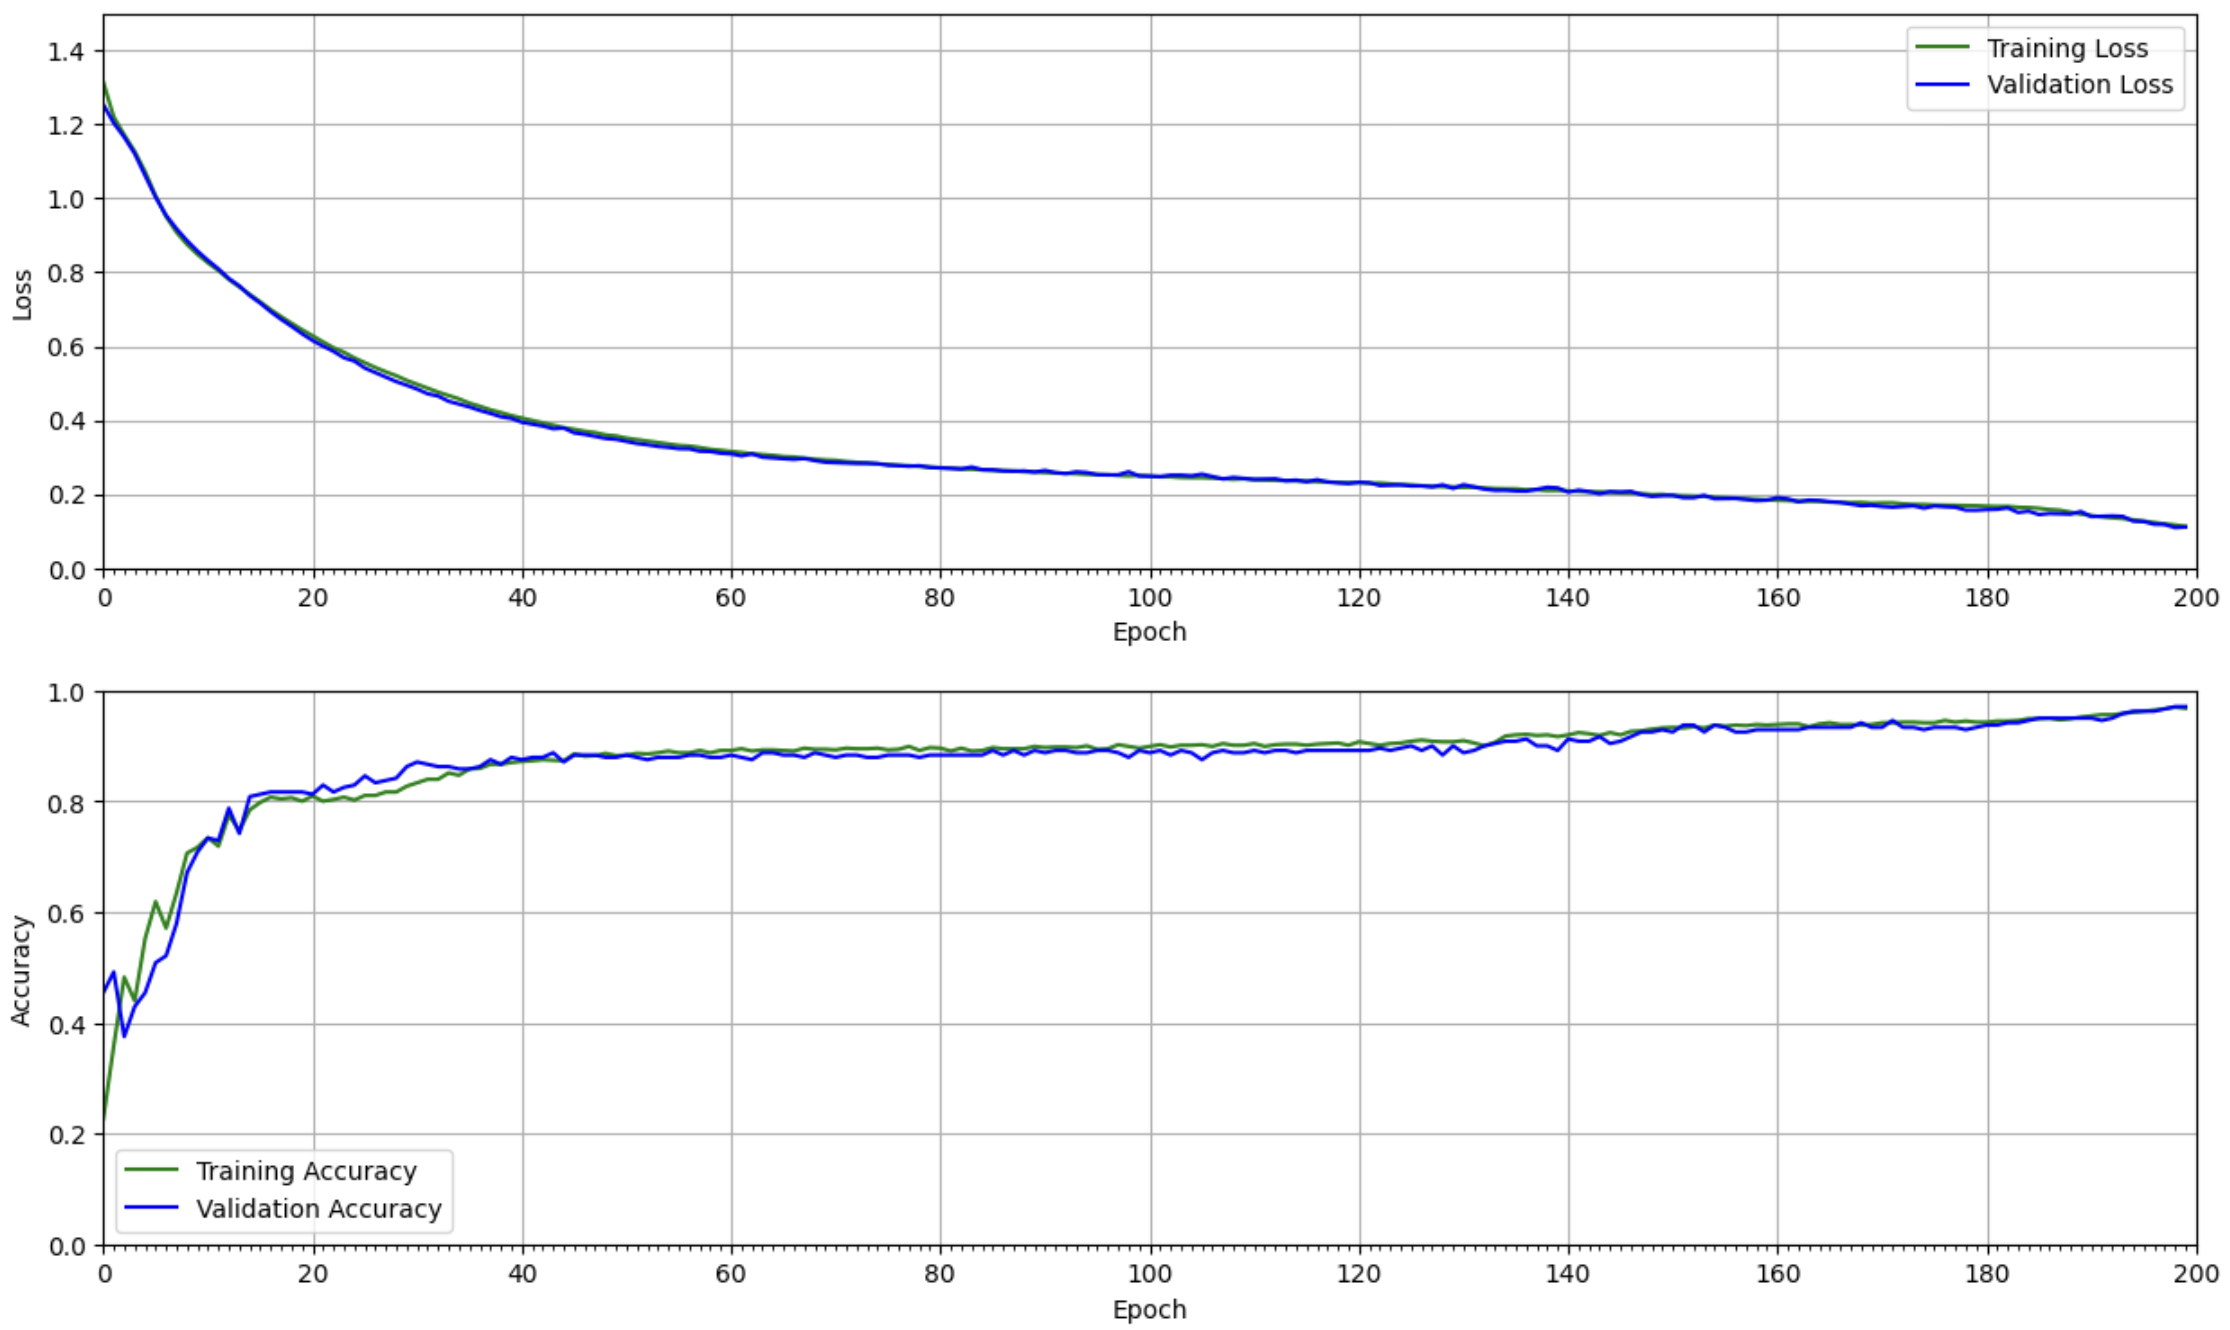
\includegraphics[width=\textwidth]{images/2.png}
	\end{center}
	\caption{Кривая обучения}
	\label{img:2}
\end{figure}

\begin{figure}
	\begin{center}
		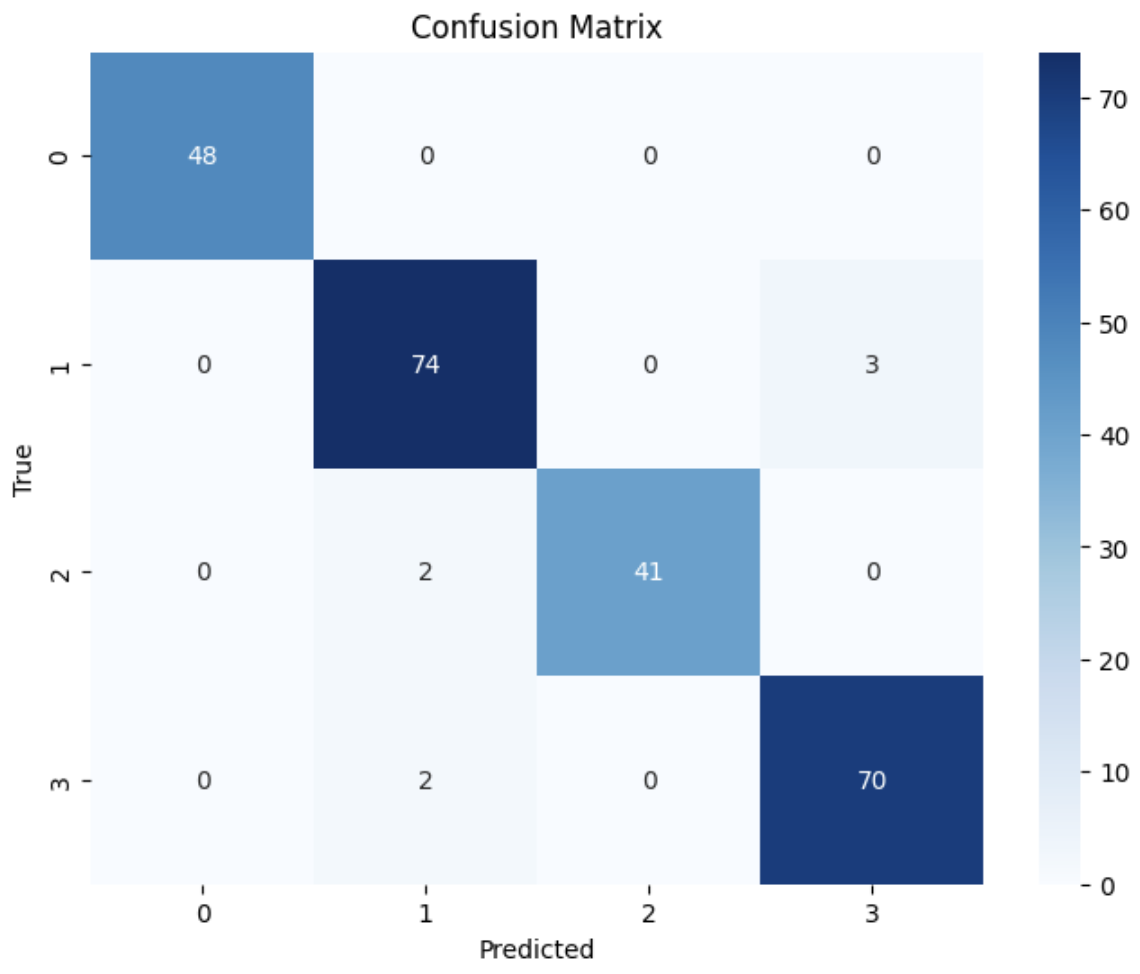
\includegraphics[width=0.7\textwidth]{images/3.png}
	\end{center}
	\caption{Матрица ошибок}
	\label{img:3}
\end{figure}

\begin{lstlisting}[label=lst:2,caption=Отчёт по результатам классификации]
	Classification Report:
							precision    recall  f1-score   support
	
	0       				1.00      1.00      1.00        48
	1       				0.95      0.96      0.95        77
	2       				1.00      0.95      0.98        43
	3       				0.96      0.97      0.97        72
	
	accuracy                            0.97       240
	macro avg     	0.98      0.97      0.97       240
	weighted avg		0.97      0.97      0.97       240
	
	Additional Metrics:
	MCC: 0.9603
\end{lstlisting}

\clearpage

\section{Использование сигмоиды (b = 1) в качестве функции активации}

\begin{figure}
	\begin{center}
		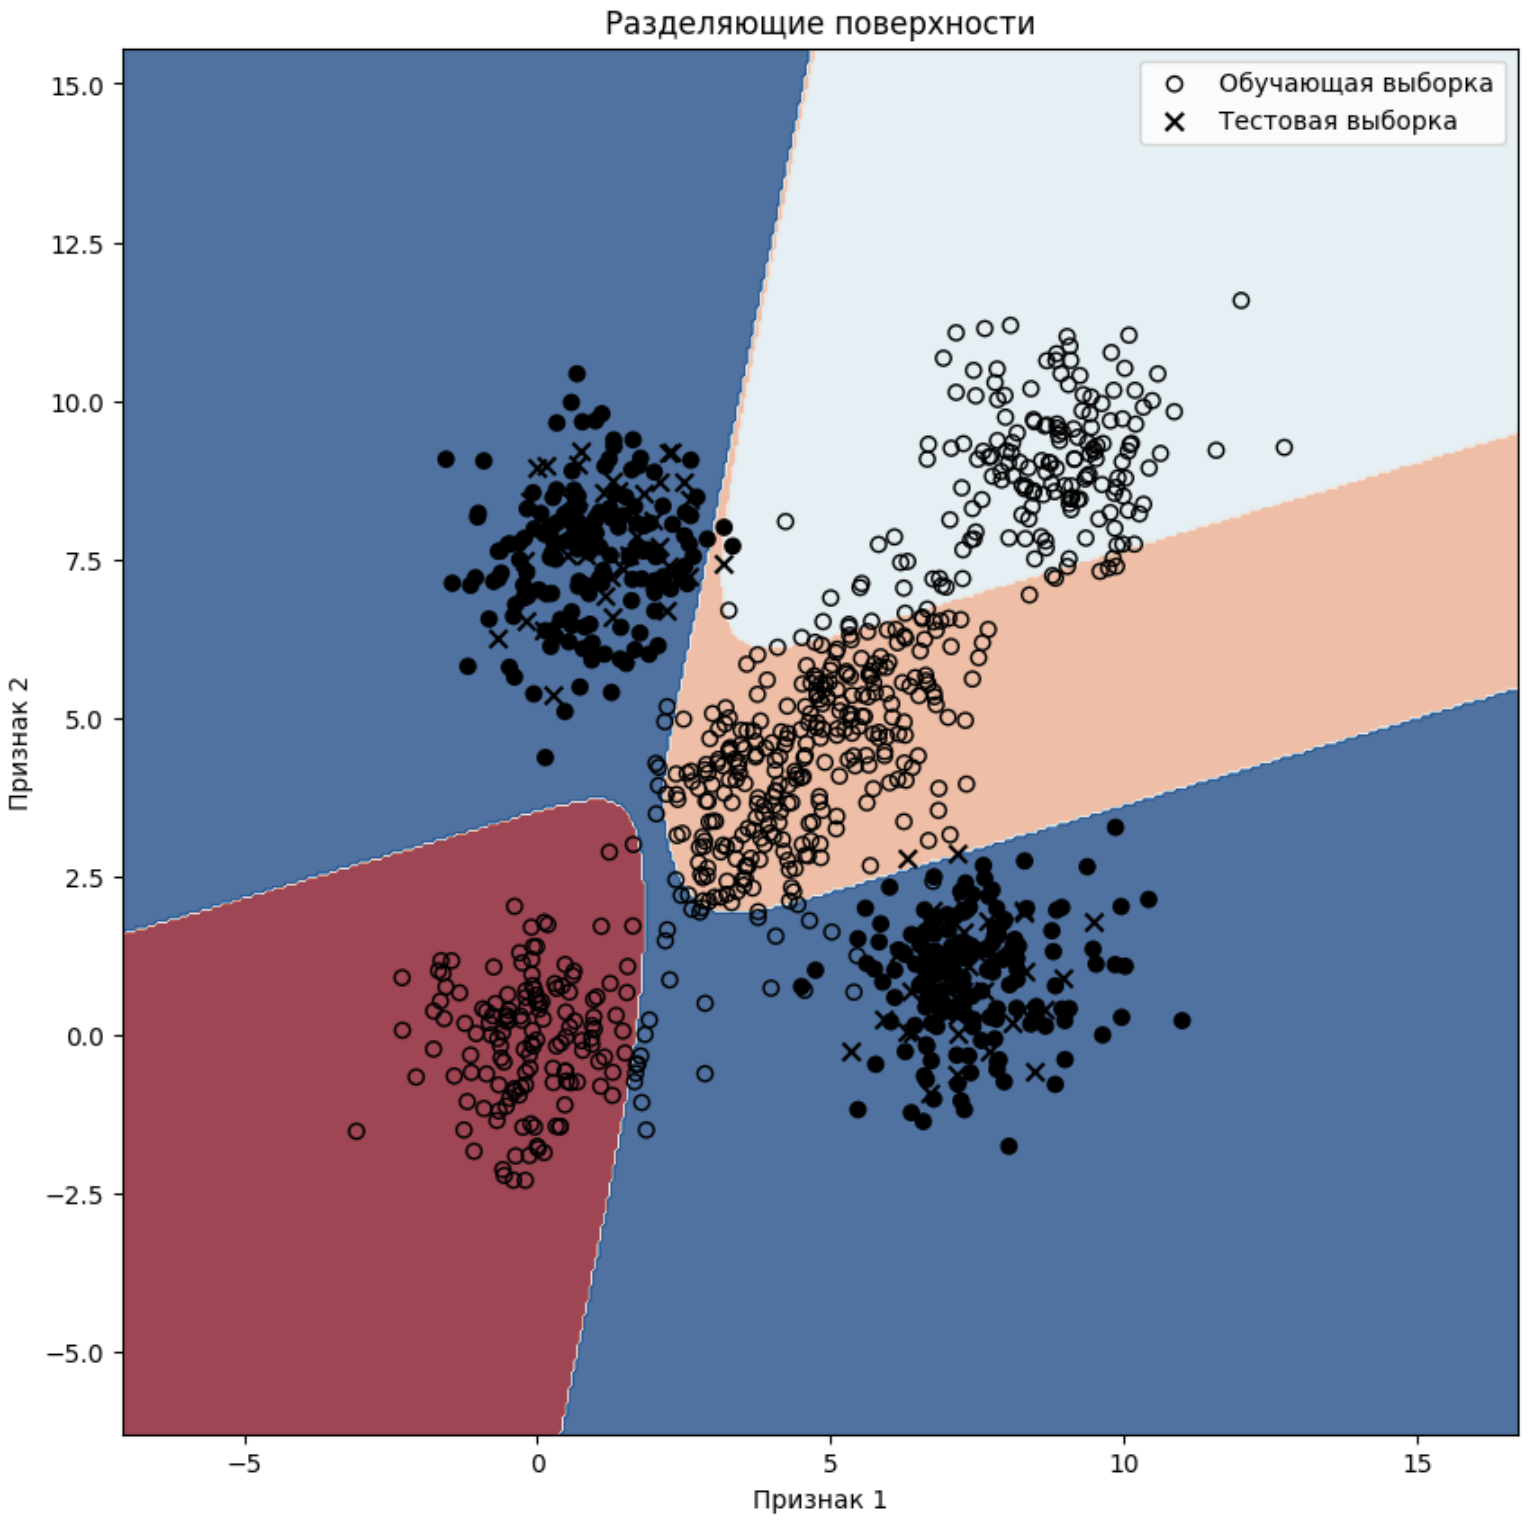
\includegraphics[width=\textwidth]{images/4.png}
	\end{center}
	\caption{Разделяющие поверхности}
	\label{img:4}
\end{figure}

\begin{figure}
	\begin{center}
		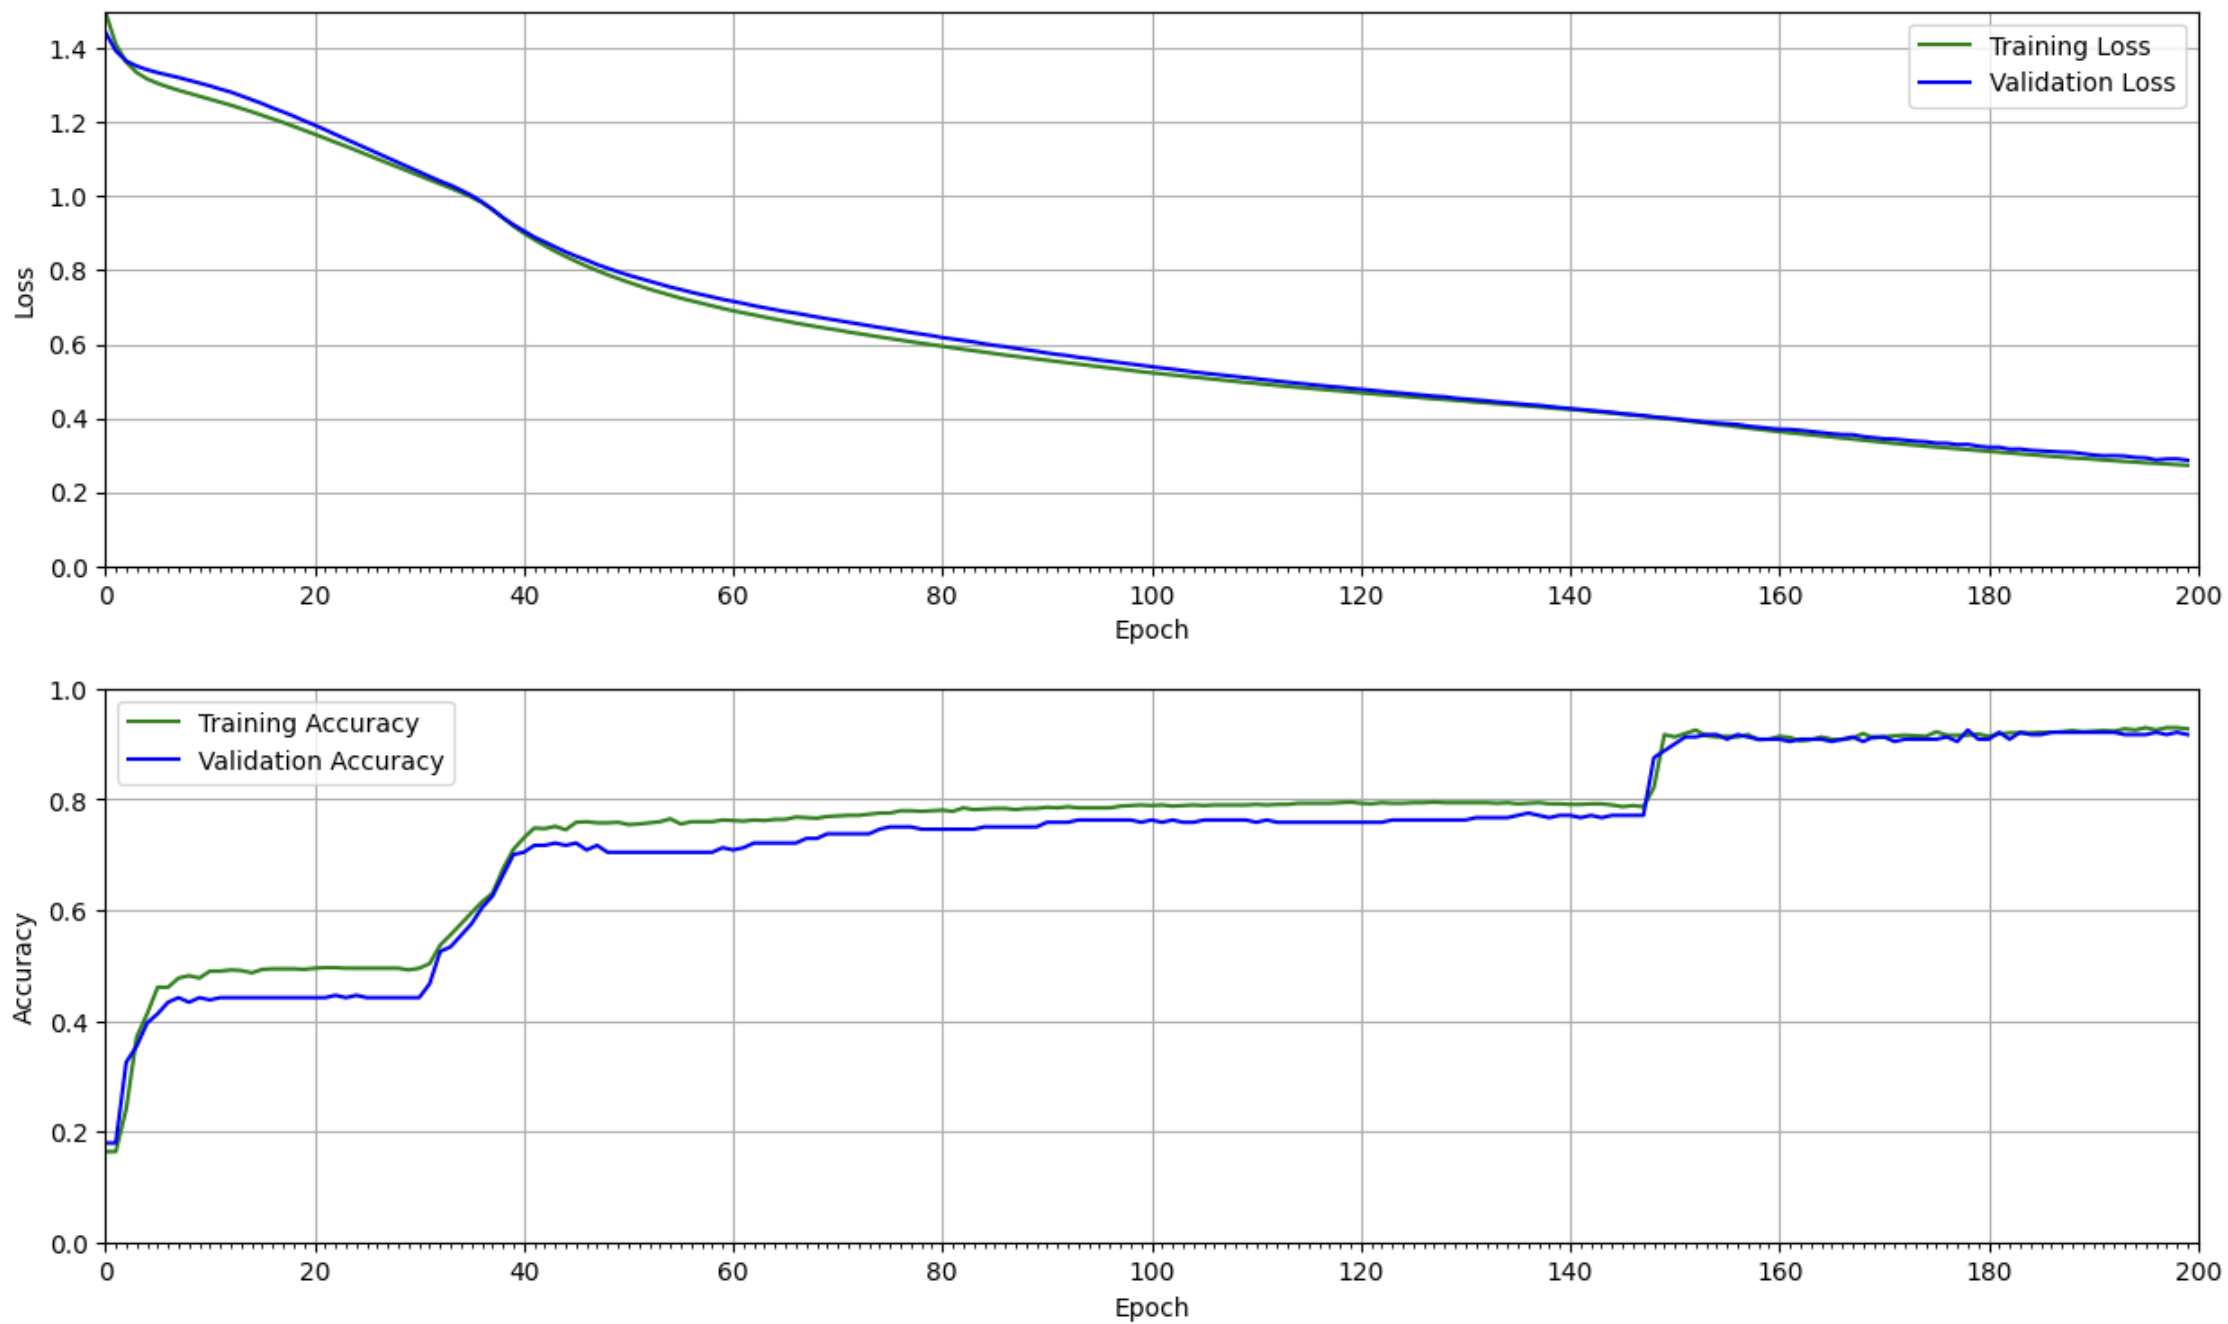
\includegraphics[width=\textwidth]{images/5.png}
	\end{center}
	\caption{Кривая обучения}
	\label{img:5}
\end{figure}

\begin{figure}
	\begin{center}
		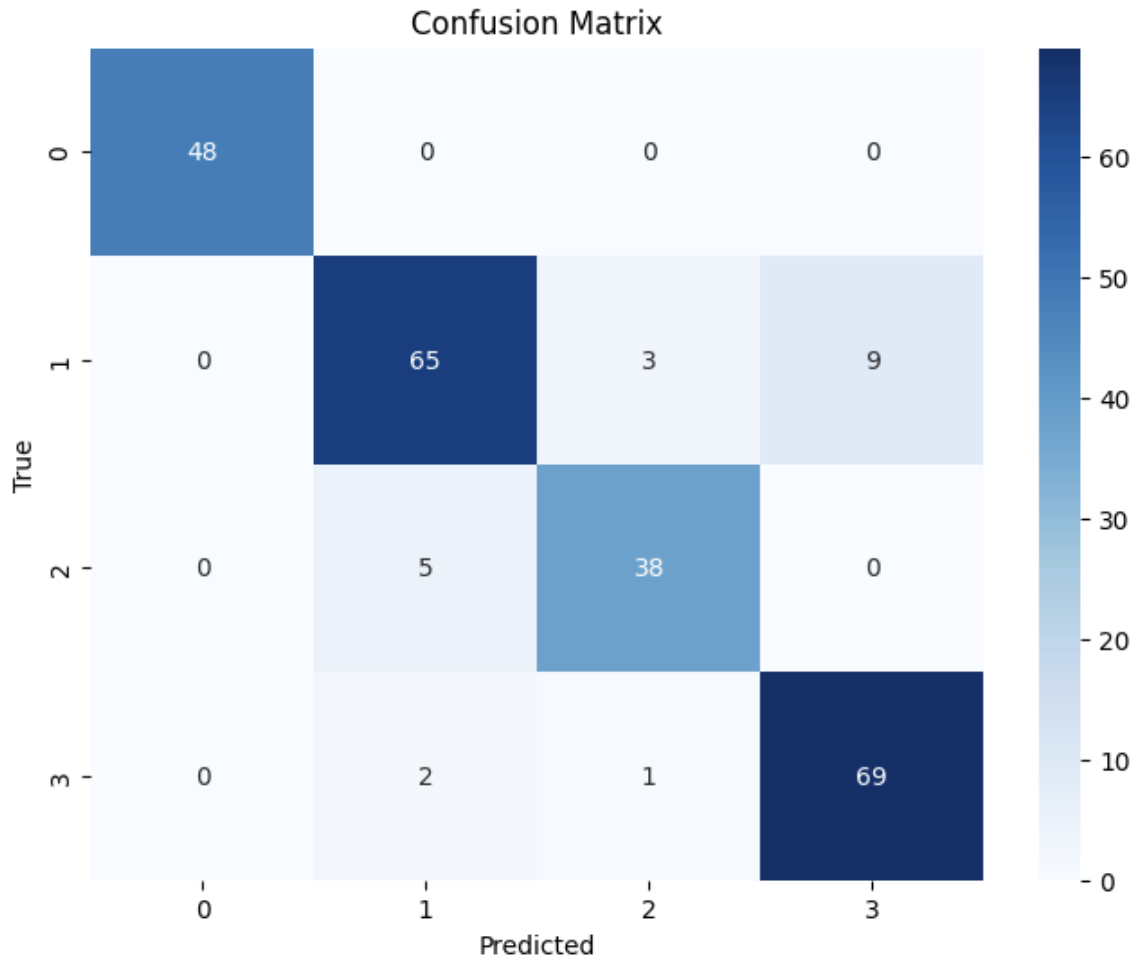
\includegraphics[width=0.7\textwidth]{images/6.png}
	\end{center}
	\caption{Матрица ошибок}
	\label{img:6}
\end{figure}

\begin{lstlisting}[label=lst:3,caption=Отчёт по результатам классификации]
	Classification Report:
							precision    recall  f1-score   support
	
	0       				1.00      1.00      1.00        48
	1       				0.90      0.84      0.87        77
	2       				0.90      0.88      0.89        43
	3       				0.88      0.96      0.92        72
	
	accuracy                           	0.92       240
	macro avg       0.92      0.92      0.92       240
	weighted avg    0.92      0.92      0.92       240
	
	Additional Metrics:
	MCC: 0.8873
\end{lstlisting}

\clearpage

\section{Использование сигмоиды (b = 5) в качестве функции активации}

\begin{figure}
	\begin{center}
		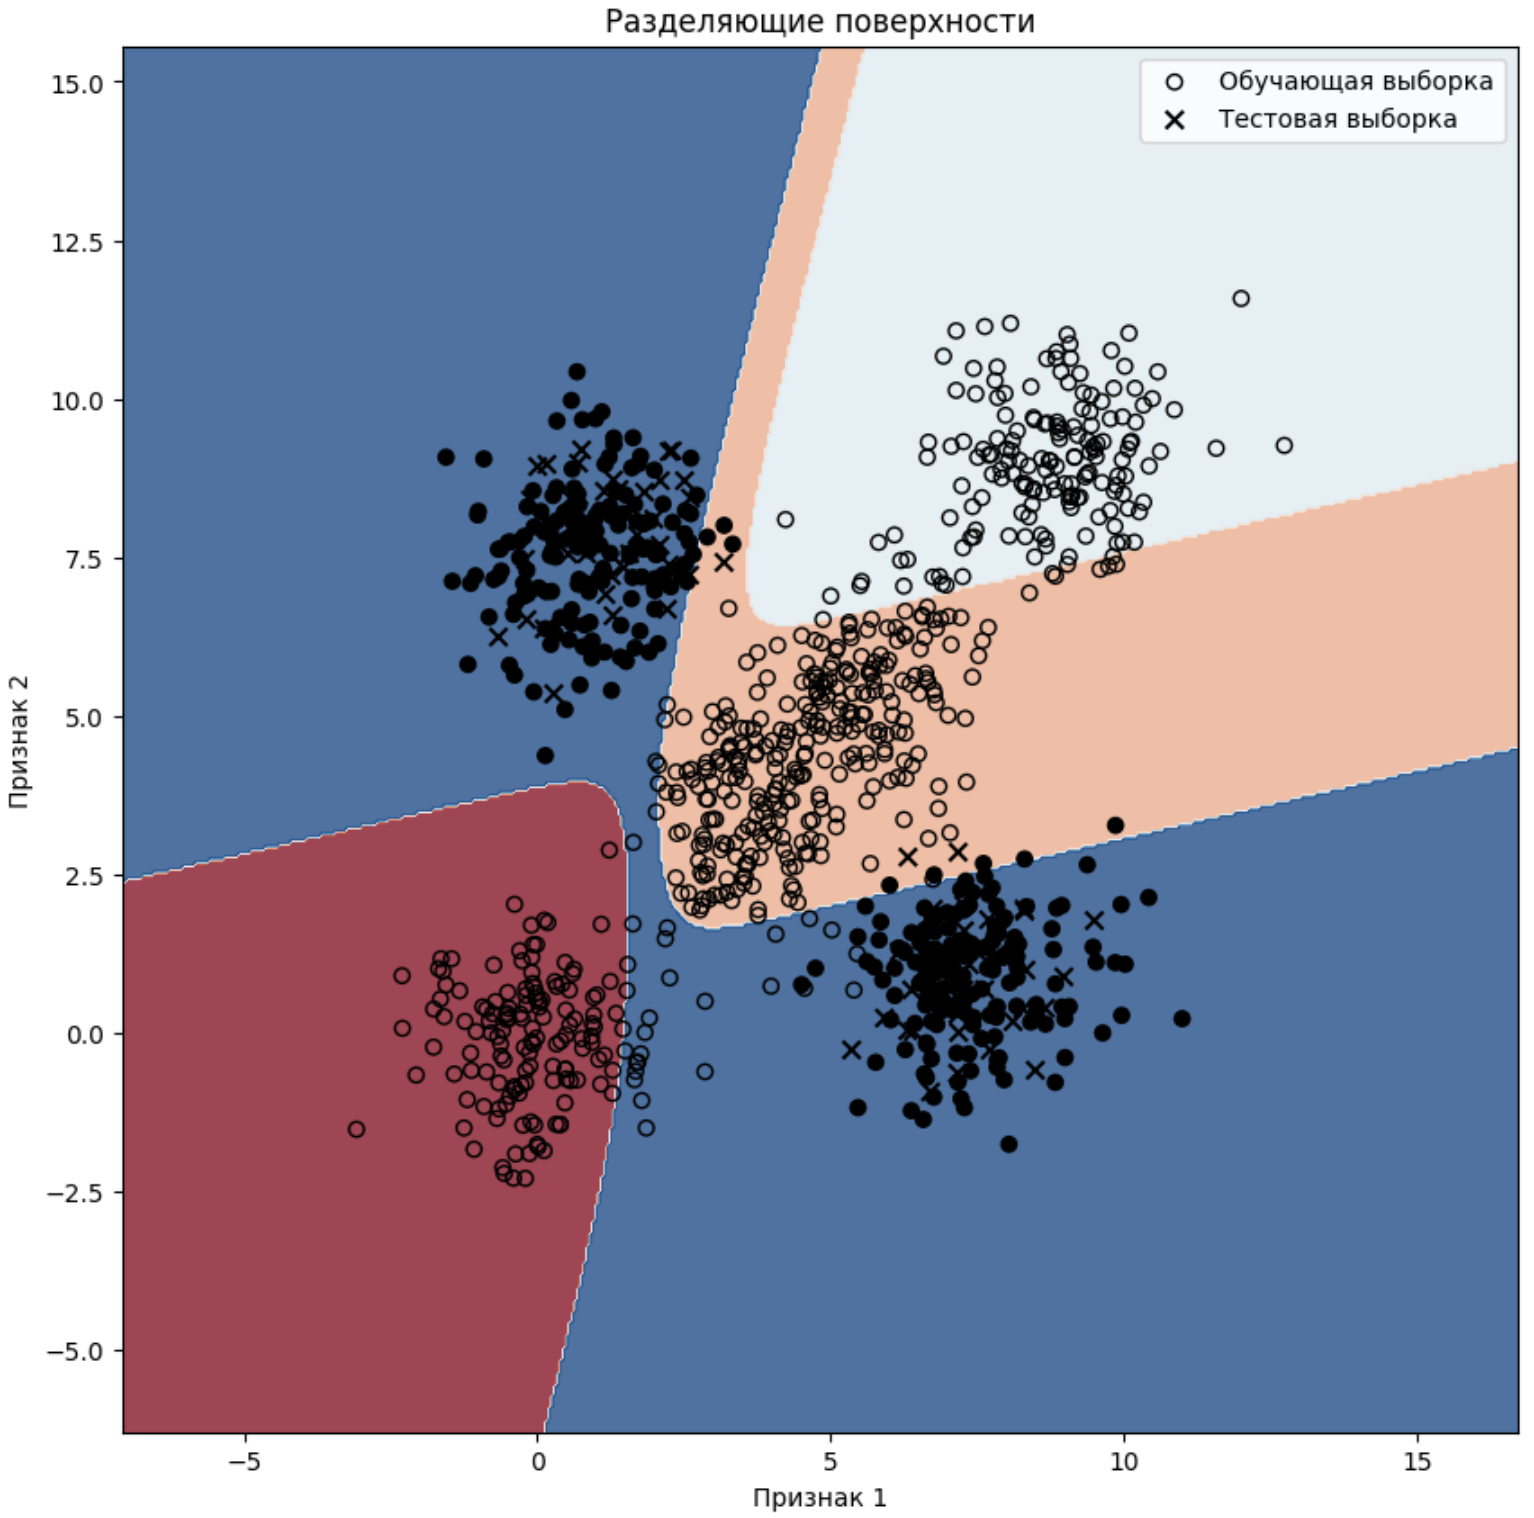
\includegraphics[width=\textwidth]{images/7.png}
	\end{center}
	\caption{Разделяющие поверхности}
	\label{img:7}
\end{figure}

\begin{figure}
	\begin{center}
		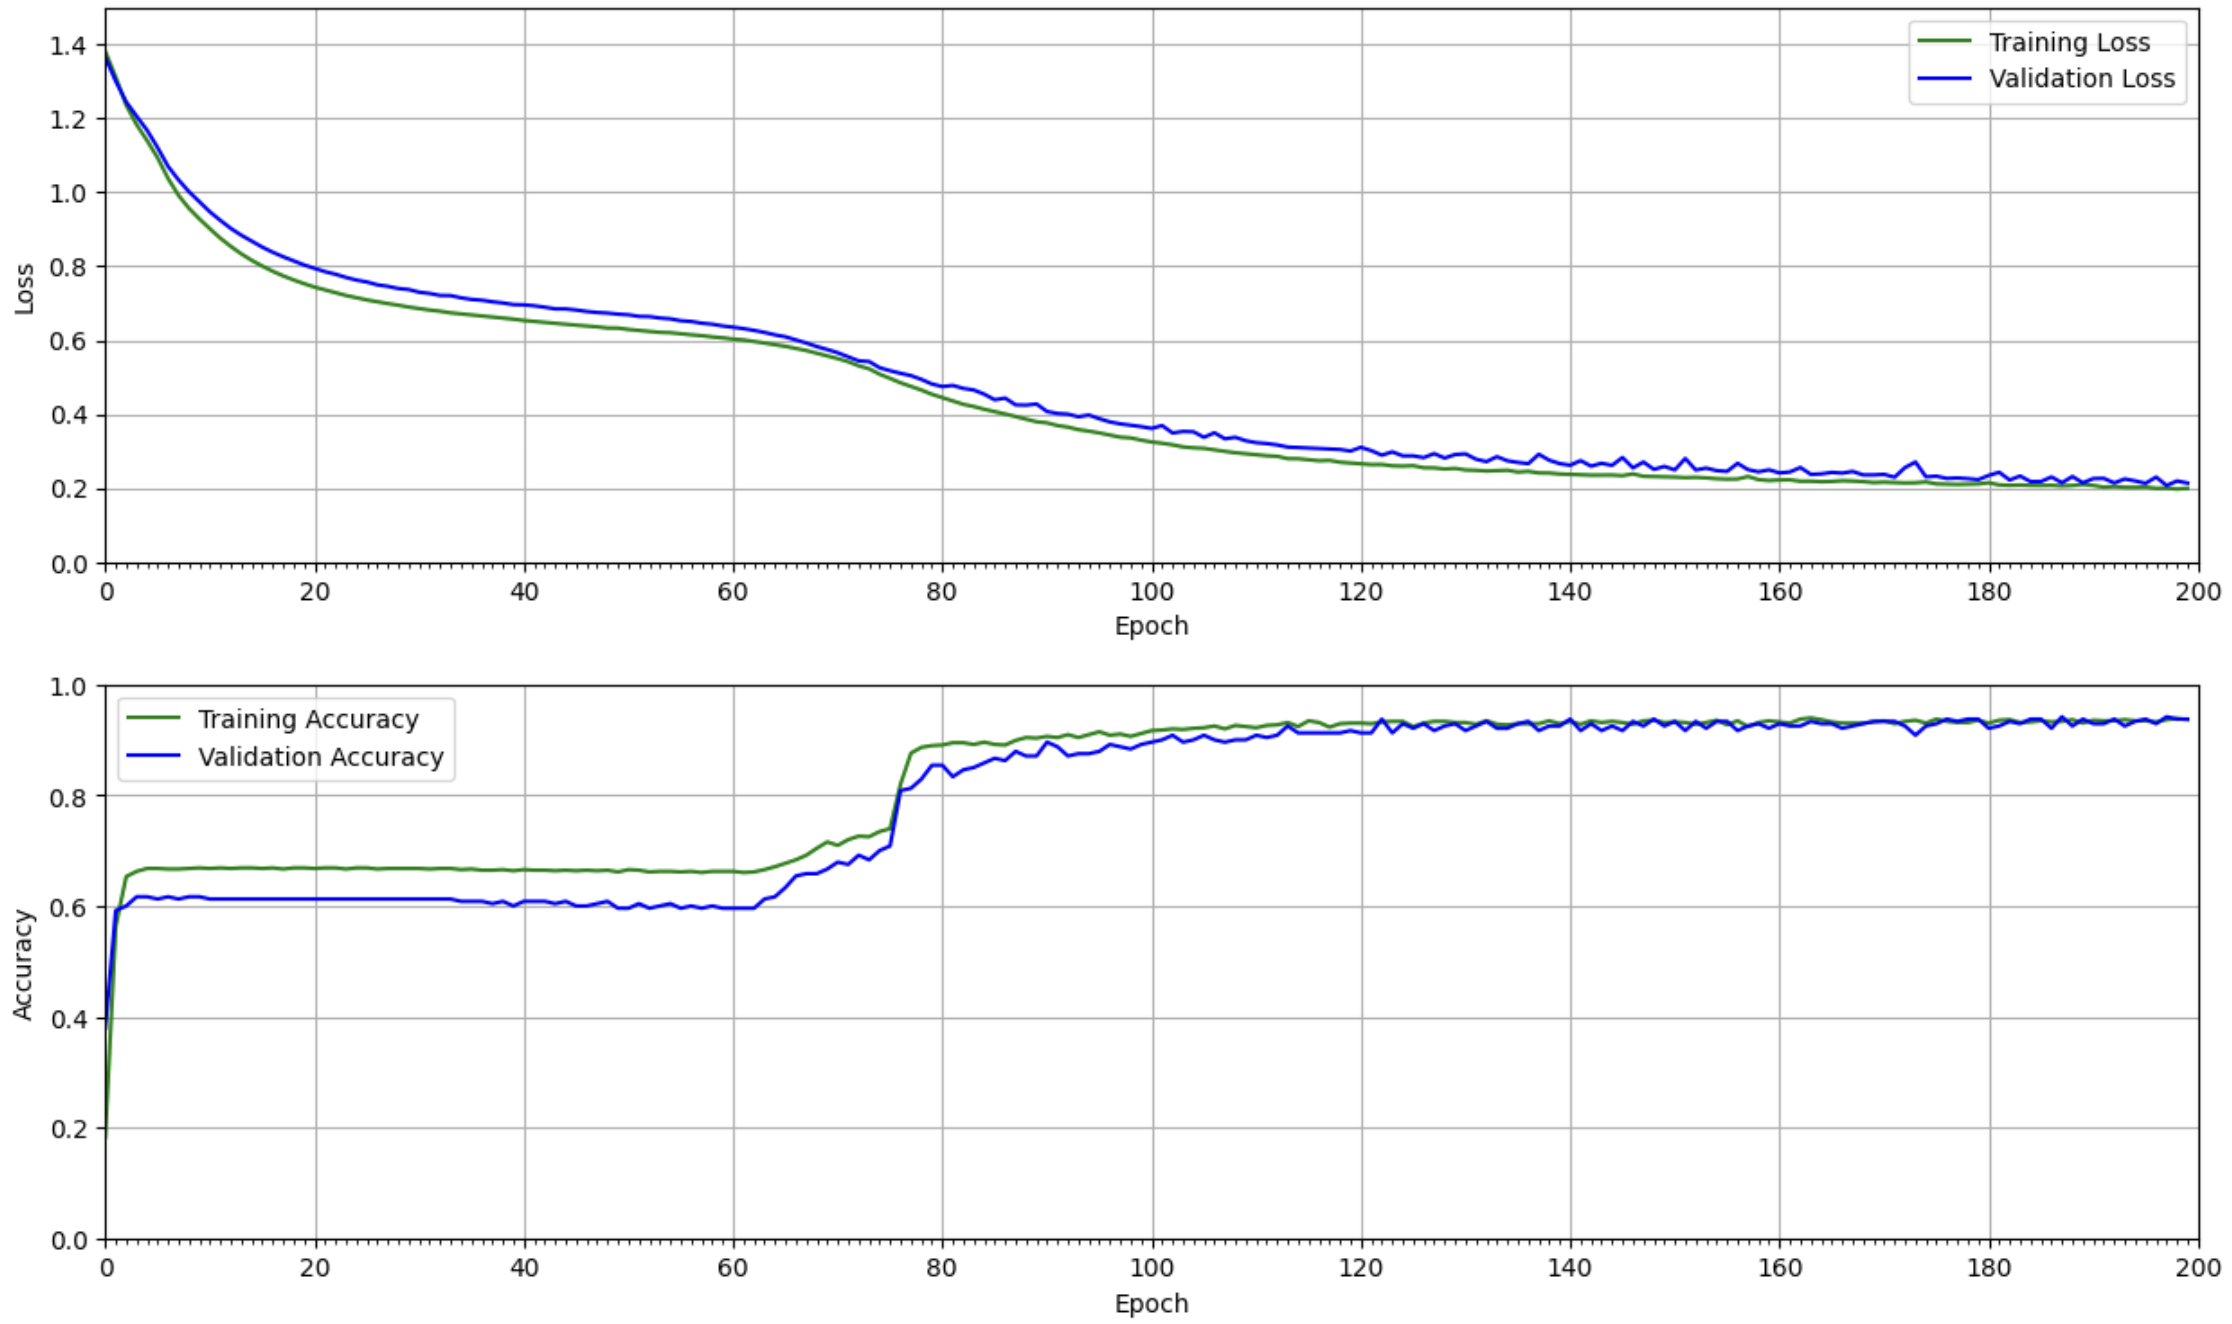
\includegraphics[width=\textwidth]{images/8.png}
	\end{center}
	\caption{Кривая обучения}
	\label{img:8}
\end{figure}

\begin{figure}
	\begin{center}
		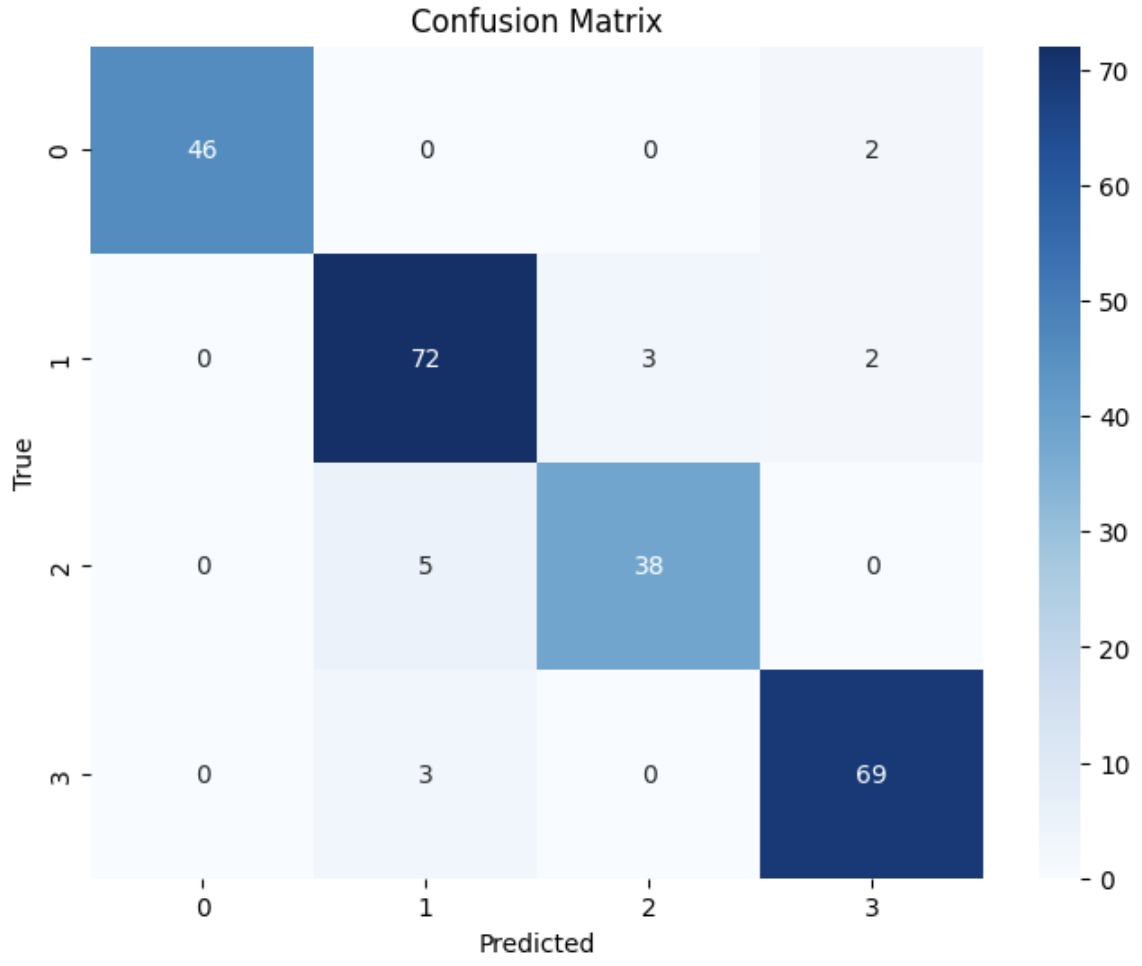
\includegraphics[width=0.7\textwidth]{images/9.png}
	\end{center}
	\caption{Матрица ошибок}
	\label{img:9}
\end{figure}

\begin{lstlisting}[label=lst:4,caption=Отчёт по результатам классификации]
	Classification Report:
							precision    recall  f1-score   support
	
	0       				1.00      0.96      0.98        48
	1       				0.90      0.94      0.92        77
	2       				0.93      0.88      0.90        43
	3       				0.95      0.96      0.95        72
	
	accuracy                           	0.94       240
	macro avg       0.94      0.93      0.94       240
	weighted avg    0.94      0.94      0.94       240
	
	Additional Metrics:
	MCC: 0.9149
\end{lstlisting}

\clearpage

\section{Использование сигмоиды (b = 10) в качестве функции активации для построения разделяющих гиперплоскостей на основе весов нейронов скрытого слоя}

\begin{figure}
	\begin{center}
		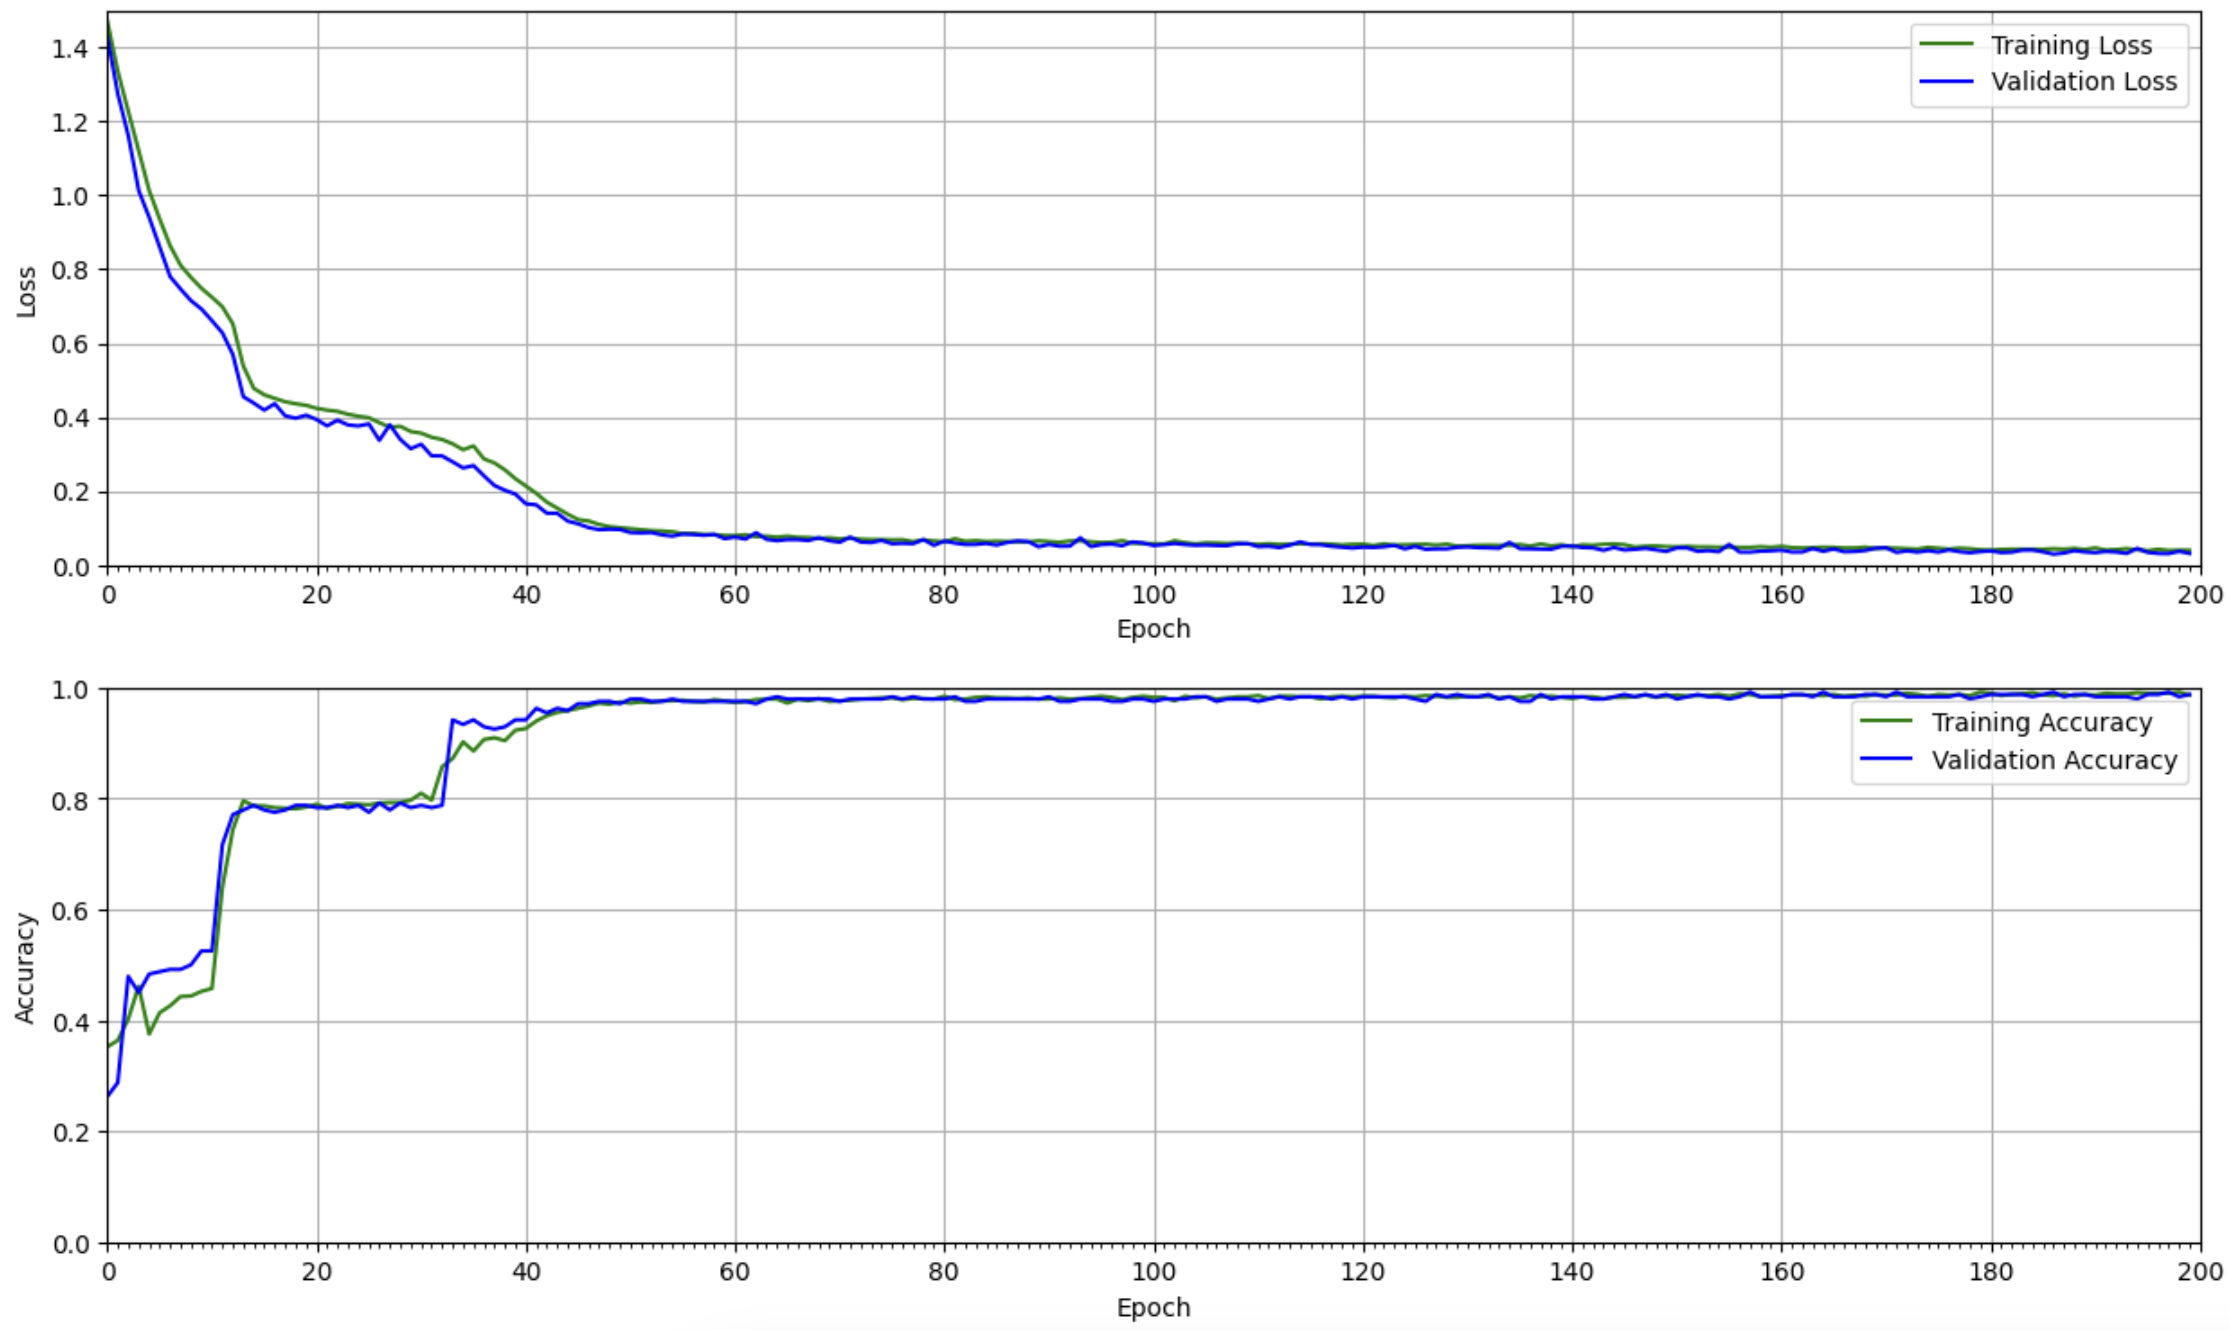
\includegraphics[width=\textwidth]{images/14.png}
	\end{center}
	\caption{Кривая обучения}
	\label{img:14}
\end{figure}

\begin{figure}
	\begin{center}
		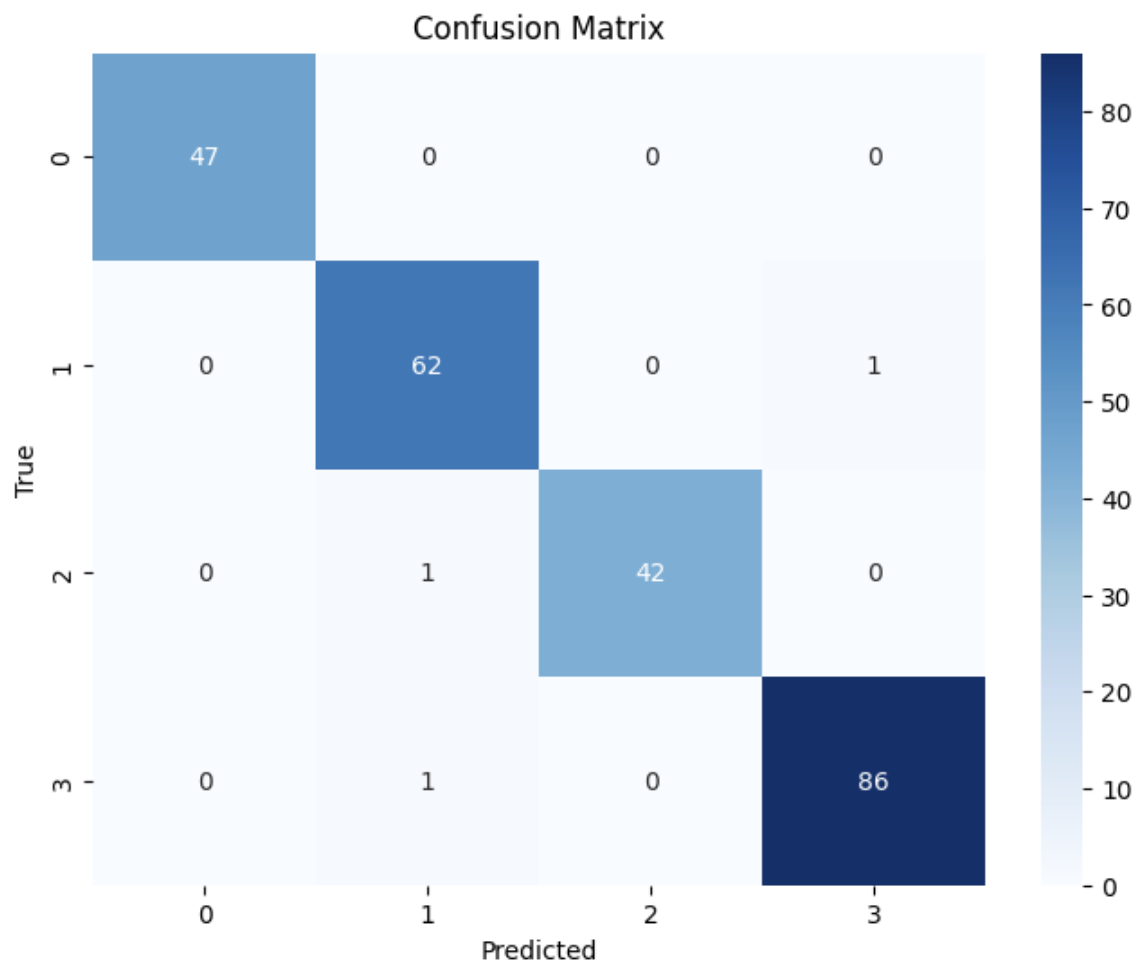
\includegraphics[width=0.7\textwidth]{images/15.png}
	\end{center}
	\caption{Матрица ошибок}
	\label{img:15}
\end{figure}

\begin{lstlisting}[label=lst:4,caption=Отчёт по результатам классификации]
	Classification Report:
							precision    recall  f1-score   support
	
	0       				1.00      1.00      1.00        47
	1       				0.97      0.98      0.98        63
	2       				1.00      0.98      0.99        43
	3       				0.99      0.99      0.99        87
	
	accuracy                            0.99       240
	macro avg     	0.99      0.99      0.99       240
	weighted avg    0.99      0.99      0.99       240
	
	Additional Metrics:
	MCC: 0.9829
\end{lstlisting}

\begin{figure}
	\begin{center}
		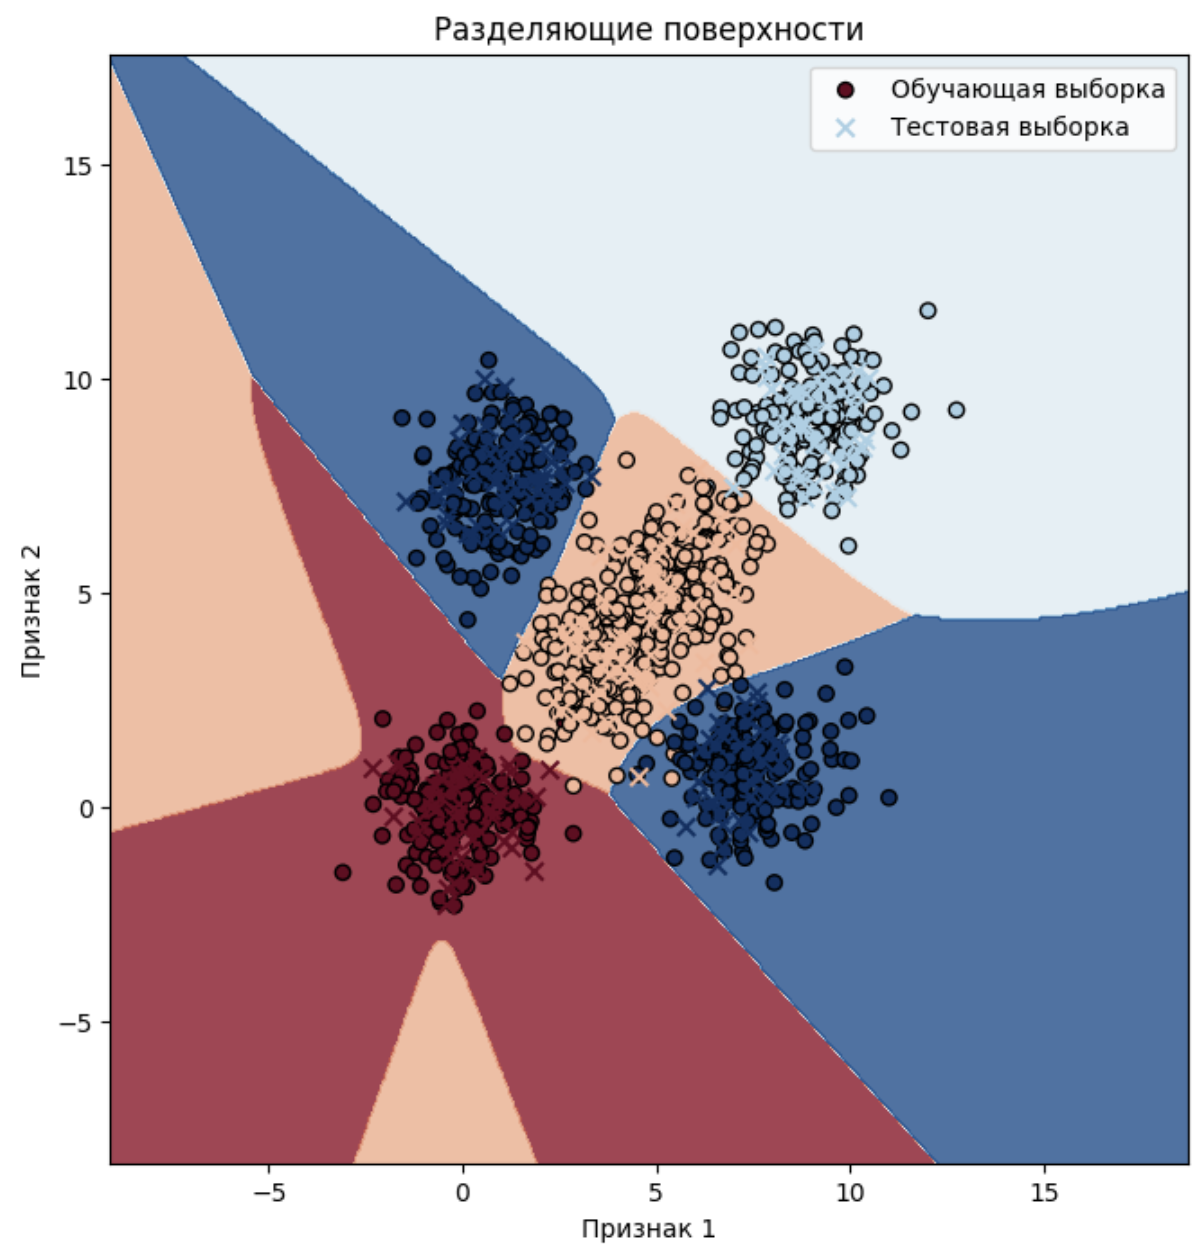
\includegraphics[width=\textwidth]{images/16.png}
	\end{center}
	\caption{Разделяющие поверхности}
	\label{img:16}
\end{figure}

\begin{figure}
	\begin{center}
		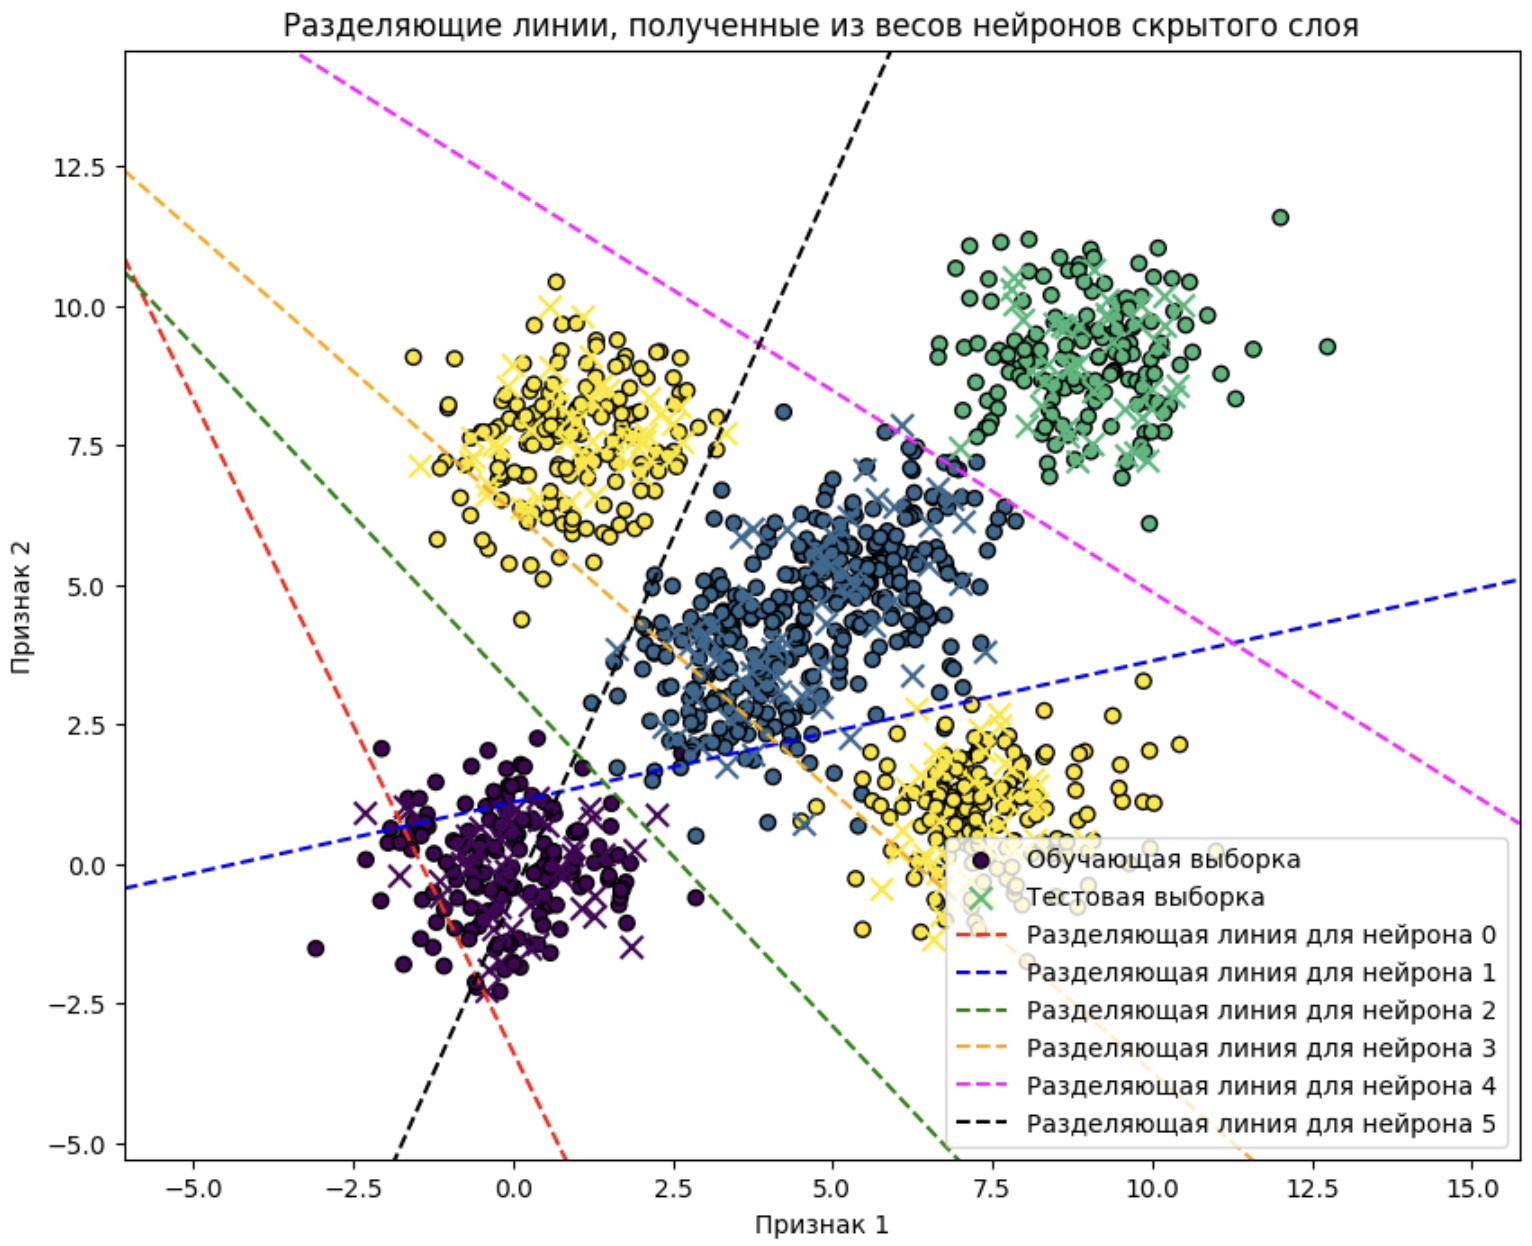
\includegraphics[width=\textwidth]{images/17.png}
	\end{center}
	\caption{Разделяющие гиперплоскости нейронов скрытого слоя}
	\label{img:17}
\end{figure}

\clearpage

\section{Добавление класса для отделения данных, далеко отстоящих от исходных классов}

\begin{figure}
	\begin{center}
		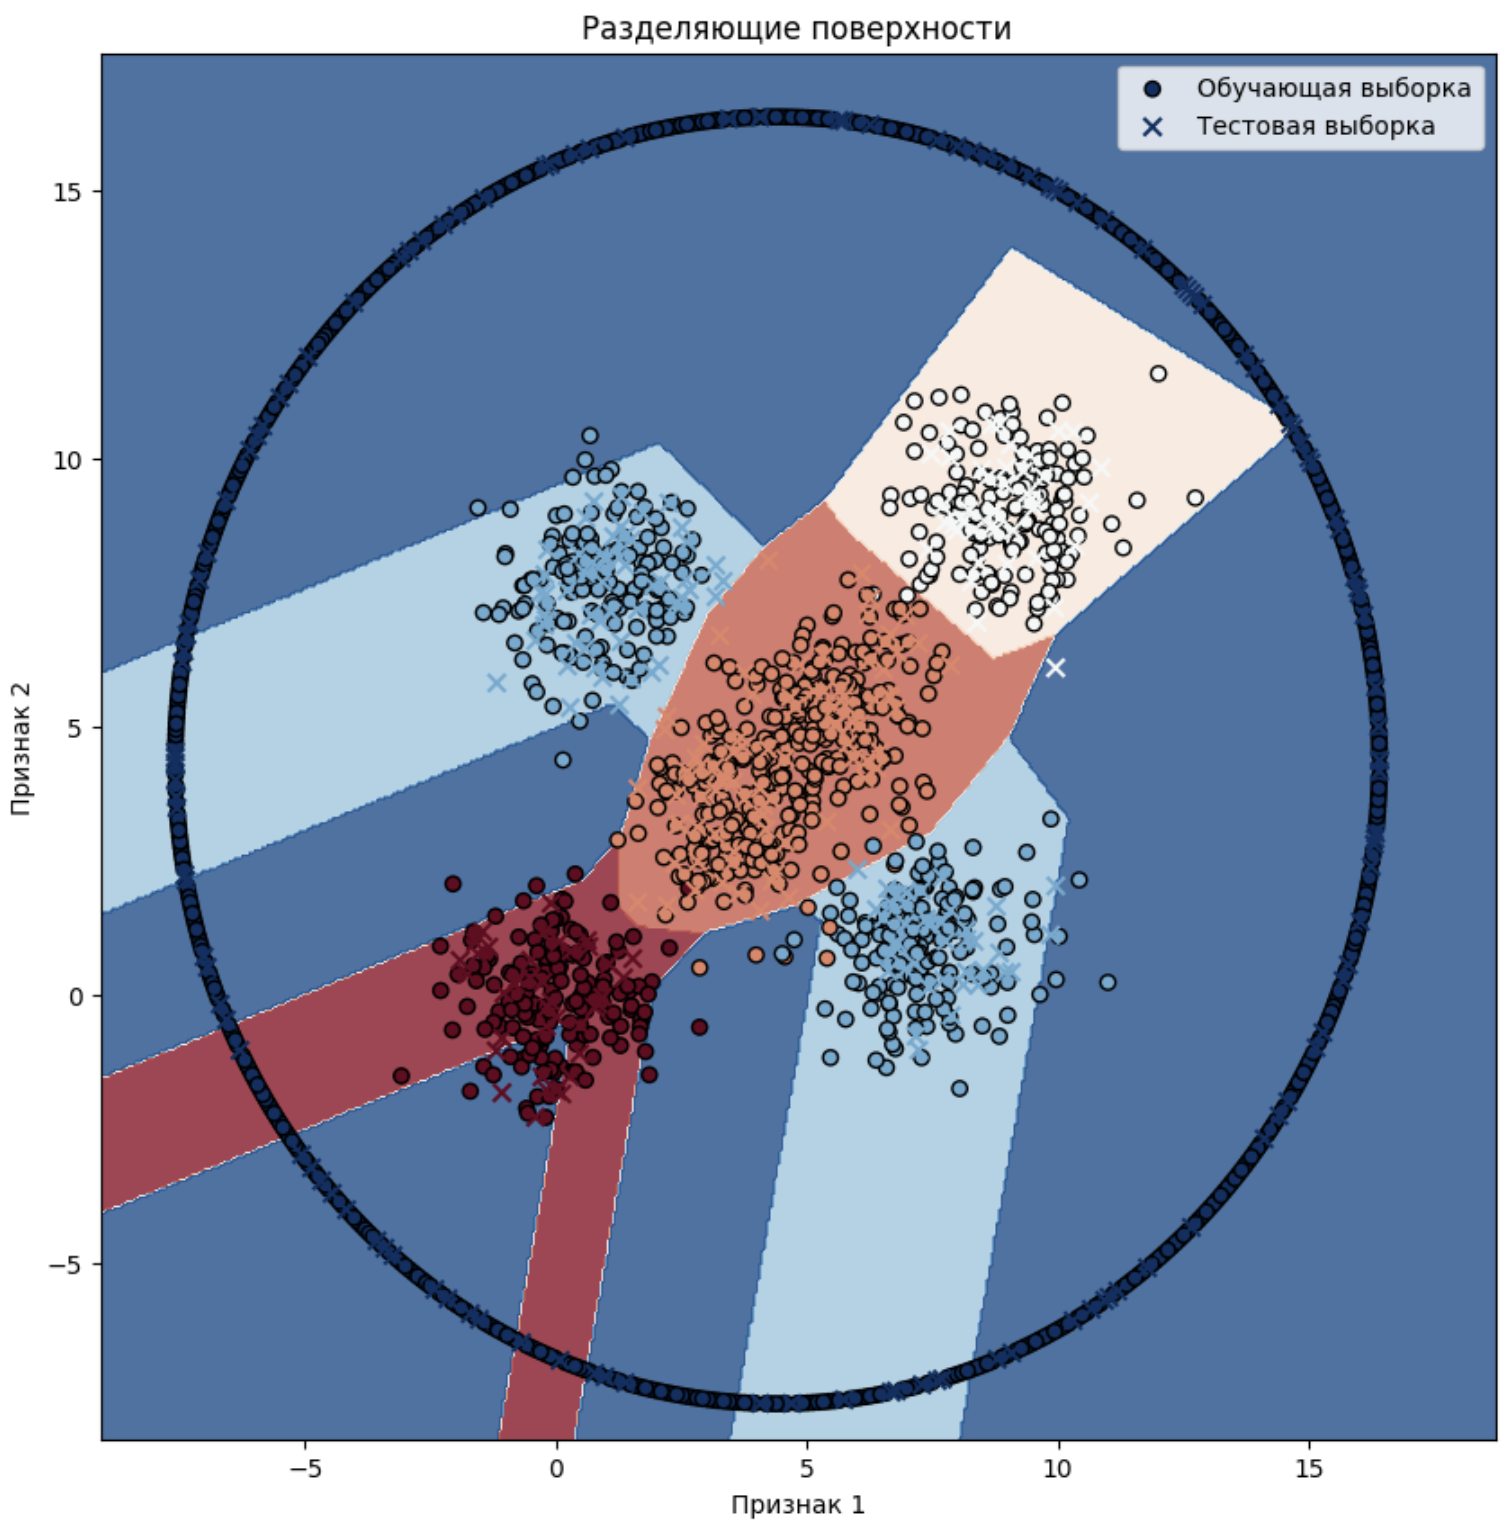
\includegraphics[width=\textwidth]{images/11.png}
	\end{center}
	\caption{Разделяющие поверхности}
	\label{img:11}
\end{figure}

\begin{figure}
	\begin{center}
		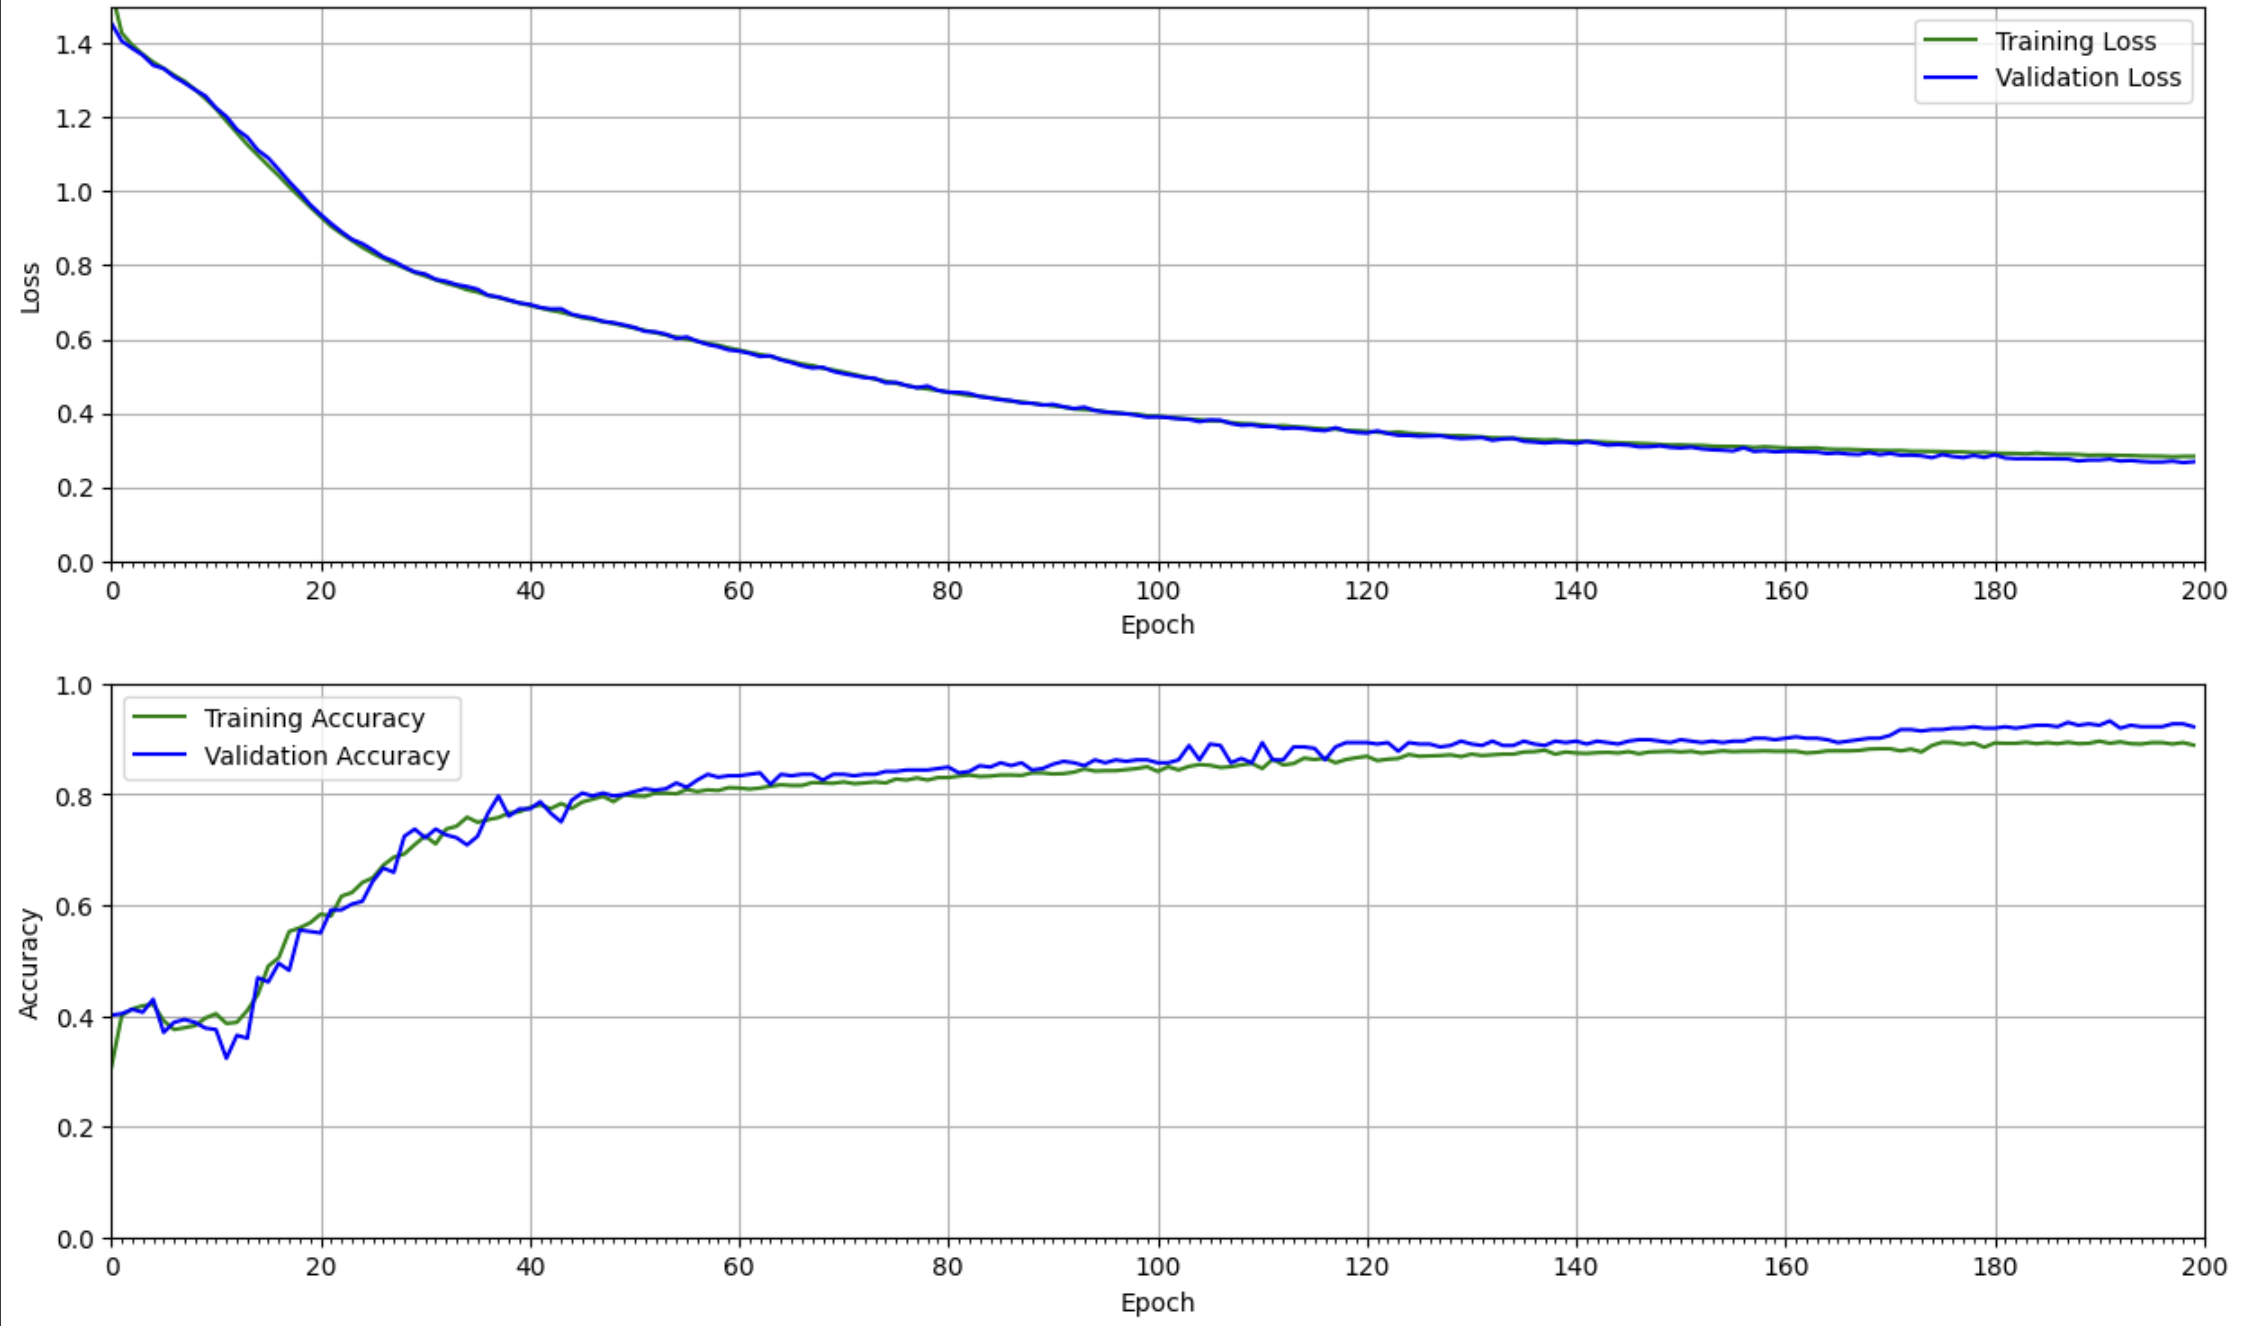
\includegraphics[width=\textwidth]{images/12.png}
	\end{center}
	\caption{Кривая обучения}
	\label{img:12}
\end{figure}

\begin{figure}
	\begin{center}
		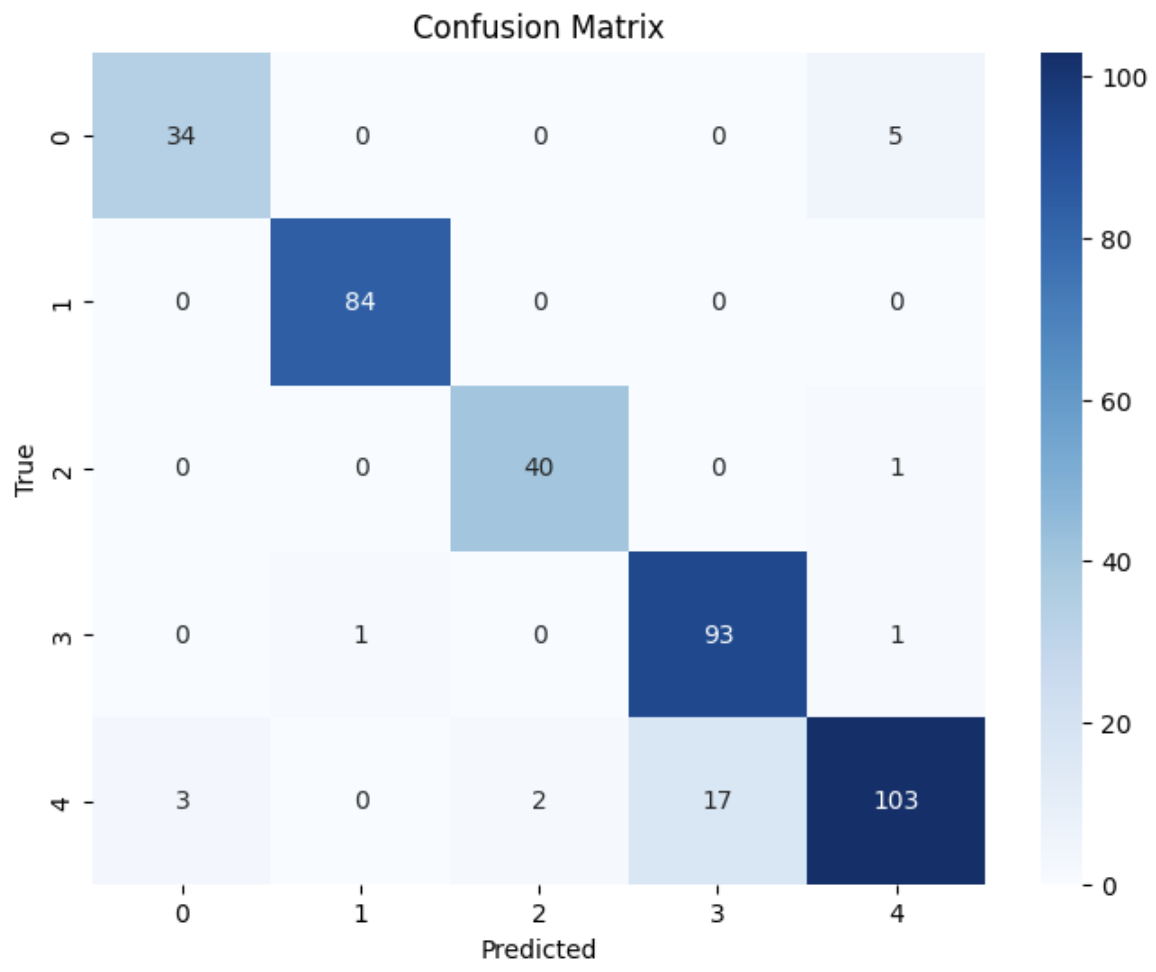
\includegraphics[width=0.7\textwidth]{images/13.png}
	\end{center}
	\caption{Матрица ошибок}
	\label{img:13}
\end{figure}

\begin{lstlisting}[label=lst:4,caption=Отчёт по результатам классификации]
	Classification Report:
							precision    recall  f1-score   support
	
	0       				0.92      0.87      0.89        39
	1       				0.99      1.00      0.99        84
	2       				0.95      0.98      0.96        41
	3       				0.85      0.98      0.91        95
	4       				0.94      0.82      0.88       125
	
	accuracy                            0.92       384
	macro avg       0.93      0.93      0.93       384
	weighted avg    0.93      0.92      0.92       384
	
	Additional Metrics:
	MCC: 0.8998
\end{lstlisting}

\clearpage
